%%% Research Diary - Entry
%%% Template by Mikhail Klassen, April 2013
%%% 
\documentclass[11pt,letterpaper]{article}
\newcommand{\workingDate}{\textsc{2018 $|$ June}}
\newcommand{\userName}{Carter Rhea}
\newcommand{\institution}{Universite de Montreal}
\usepackage{python}

\usepackage[]{algorithm2e}
\usepackage{subcaption}
\usepackage{listings}
\usepackage{color}
\definecolor{dkgreen}{rgb}{0,0.6,0}
\definecolor{gray}{rgb}{0.5,0.5,0.5}
\definecolor{mauve}{rgb}{0.58,0,0.82}
\usepackage{hyperref}
\hypersetup{
	colorlinks=true,
	linkcolor=blue,
	filecolor=magenta,      
	urlcolor=cyan,
}
\lstset{frame=tb,
	language=Java,
	aboveskip=3mm,
	belowskip=3mm,
	showstringspaces=false,
	columns=flexible,
	basicstyle={\small\ttfamily},
	numbers=none,
	numberstyle=\tiny\color{gray},
	keywordstyle=\color{blue},
	commentstyle=\color{dkgreen},
	stringstyle=\color{mauve},
	breaklines=true,
	breakatwhitespace=true,
	tabsize=3
}
\usepackage{researchdiary_png}
% To add your univeristy logo to the upper right, simply
% upload a file named "logo.png" using the files menu above.

\begin{document}
\univlogo

\title{Documentation for WVT}

%\begin{python}%
%print r"Hello \LaTeX!"
%\end{python}%
\textit{Documentation for my Weighted Voronoi Tessellations Algorithm.}

\tableofcontents

\newpage


\newpage
\section{Weighted Voronoi Tessellations}

\subsection{Introduction}
Before delving into Weighted Voronoi Tessellations, I would first like to simply describe why we care about them (other than the fact that they are pretty cool). In a few words: WVT allows for a binning scheme that is unbiased when compared with Voronoi Tessellations, Centroidal Voronoi Tesselations, or other binning methods. Once we have the WVT bins in place, we can use that information to general temperature maps for X-ray data (That's what I am interested in).

See \cite{Copin2018}, \cite{Diehl2008}, and \cite{Sanders2018} for more information.
\subsection{Signal-to-Noise}
For our particular application in X-ray astronomy, we are going to be interested in a signal-to-noise ratio dominated by count rates. Count Rates are a relatively easy quantity for us to compute.
The following equation are for pixel number $k$.
\begin{equation}\label{eqn:signal}
	Signal_k = Flux_k = \frac{C_k}{E_k \tau}-B_k
\end{equation}
\begin{equation}\label{eqn:noise}
	Noise_k = \sigma^2_k = \frac{C_k}{E^2_k\tau^2}+\sigma^2_{B_k}
\end{equation}

\begin{center}
	\begin{tabular}{|c|c|}
		\hline 
		Parameter & Definition \\
		\hline
		\hline
		$C_k$ & Raw Counts \\
		\hline 
		$E_k$ & Effective Area \\
		\hline 
		$\tau$ & Exposure Time \\
		\hline
		$B_k$ & Background Flux \\
		\hline 
		$\sigma_{B_k}$ & Uncertainty in Background Flux \\
		\hline
	\end{tabular}
\end{center}

\begin{equation}
B_k = \frac{\bar{C}_B}{E_k*\tau}
\end{equation}
with $\bar{C}_B$ being the average background counts.

$\sigma_{B_k}$ is just the $1-sigma$ error value for $B_k$.

\textbf{CURRENTLY BACKGROUND IS NOT TAKEN INTO ACCOUNT}

This calculation and data-gathering occurs in the \textsc{read\_in} subroutine. 

That sums up signal-to-noise calculations in the current version of the code.

\subsection{Algorithm Run-Down}
This section will contain the pseudo-algorithm of my python code.

Before we are able to begin our algorithm (WVT) in earnest, we must have a decent initial guess! 

Enter \textbf{Bin Accretion}....
\subsubsection{Bin Accretion}
\begin{algorithm}[H]\label{algo:BA}
	\caption{Bin Accretion Algorithm}
	\KwData{Pixels}
	\KwResult{Initial Guess for WVT}
	initialization\;
	\While{Pixels left to be assigned}{
		\While{Criteria not all met}{
			Calculate pixel closest to bin centroid\;
			Calculate Adjacency\;
			Calculate Roundness\;
			Calculate Potential Signal-to-Noise\;
			\eIf{Criteria all met}{
				Add pixel to Bin\;
			}{
				Start new bin\;
			}
			\If{Signal-to-Noise too low}{
				Mark pixels unassigned\;
			}		
		}
	}
	Reassign all unassigned pixels to nearest bin\;
\end{algorithm}

With that out of the way we can discuss how I actually calculated the three different criteria: Adjacency, Roundness, Potential Signal-to-Noise.

\begin{itemize}
	\item Adjaceny: This one is simple: just check if the pixels are neighbors!
	\item Roundness: Ok so now we finally need to calculate some stuff... More explicity $R_{equiv}$ and $R_{max}$. $R_{max}$ is the maximum distance from the centroid for ALL pixels in bin. $R_{equiv}$ is a wonderfully horrendous quantity which is "the radius of a disk around the bin". Lets do a quick little derivation...
	\begin{equation}
		Area_{circle} = \pi r_{circle}^2 == n\pi\frac{d_{pix}}{2}^^2 = Area_{bin}
	\end{equation} 
	Solving for $r_{circle}$ we get,
	\begin{equation}
		r_{circle} = \sqrt{\frac{n}{\pi}} \ d
	\end{equation}
	And now we can calculate the roundness parameter which describes the compactness of the bin:
	\begin{equation}
		Roundness = \frac{R_{max}}{R_{equiv}} - 1
	\end{equation}
	We generally shoot for a value of $Roundness = 0.3$.
	\item Potential Signal-to-Noise: We add the pixel to the bin and then recompute the Signal-to-Noise. This needs to be less than the target Signal-to-Noise.
\end{itemize}

And now to the main event (which is not very much coding wise compared to bin accretion).

\subsubsection{WVT}
\begin{algorithm}[H]\label{algo:BA}
	\caption{Weighted Voronoi Tessellation Algorithm}
	\KwData{Bins}
	\KwResult{WVT Data}
	initialization $-->$ read in Bin Accretion Data\;
	\While{Bins not converged}{
		\For{bin in Bins}{
		Recalculate Signal-to-Noise\;
		Calculate Area\;
		Calculate Centroid\;
		Calculate Scale Length\;
		}
		Reassign Pixel to Closest Bin\;
	}
\end{algorithm}
And again we need to define two properties: Area and Scale Length.
\begin{itemize}
	\item Area: Area of bin. This is basically just the area of the pixels in the bin...
	\begin{equation}
		A_{bin} = (Pixel\_Length)^2*N_{pixels} 
	\end{equation}
	\item Scale Length: This scale length is the KEY to the WEIGHTED part of WVT.
	\begin{equation}
		\sqrt{\frac{A_{bin}}{\pi}\frac{S/N}{(S/N)_{target}}}
	\end{equation}
\end{itemize}

And really thats it!

\newpage


\section{Preprocessing of Data and Selection of Inputs}
I finally decided to put this section as the second chapter since the main goal of this document is to outline the WVT algorithm. However, I also wanted to include this information for anyone interested in X-ray data reduction from \textit{CHANDRA}.

\textbf{More importantly, this section follows the steps necessary to create all the inputs for the WVT algorithm.}

\subsection{Download Data}
Before we can begin to preprocess the data, we obviously need to have the data. Thankfully, this is incredibly simple! After downloading the data from the chandra website or using $$download\_chandra\_obsid \ \#OBSID $$ 
There exists a considerable amount of documentation on each file downloaded at 
$$\href{http://cxc.harvard.edu/ciao/threads/intro_data/}{http://cxc.harvard.edu/ciao/threads/intro\_data/} $$
\subsection{Reduce Data}
We reduced the data with the following command: $$chandra\_repro $$
For details on what the reprocessing does visit the following website:
$$\href{http://cxc.harvard.edu/ciao/ahelp/chandra_repro.html}{http://cxc.harvard.edu/ciao/ahelp/chandra\_repro.html}$$



\subsection{Region of Interest}
Once we have the reduction completed, we can move onto dealing with the data we are interested in...

\textbf{MUST BE RECTANGULAR REGION FILES}

Create your region of interest as such...
\begin{itemize}
	\item opened ds9 and picked the region of interest: "ds9 ...evt2.fits \&" and RofI is called "simple.reg"
	\item Also created background image "simple\_bkg.reg"
\end{itemize}

We must save the \textit{simple.reg} as standard, \texttt{ftk5}, units \textbf{AND} in \texttt{IMAGE} units. Save the \texttt{IMAGE} coordinate region file as \textit{simple\_imcoord.reg}.

\subsection{Create Fits Files and Exposure Map}

At this point, we have all inputs necessary to run another python file: \texttt{Precursor.py} -- found in \textbf{AstronomyTools/GeneralUse}. Running this tool will create both fits files for the region of interest and the exposure map. If you opt to not use \texttt{Precursor.py}, run the following commands...


Now we must create an image-fits file by running the following commands:
\begin{lstlisting}
dmcopy "acisf#####_repro_evt2.fits[sky=region(simple.reg)]" simple.fits
dmcopy "simple.fits[events][bin x=::.1,y=::.1][IMAGE]" simple_img.fits
dmcopy "acisf#####_repro_evt2.fits[sky=region(simple_bkg.reg)]" simple_bkg.fits
dmcopy "simple_bkg.fits[events][bin x=::.1,y=::.1][IMAGE]" simple_bkg_img.fits
\end{lstlisting}

And now we create the exposure map with the following command....

\begin{lstlisting}
	fluximage "simple.fits" outroot=flux bands=broad binsize=1 units=area clobber=yes cleanup=no
\end{lstlisting}

Now we move on to the other inputs....
\begin{itemize}
	\item StN\_Target - This is a user chosen value for the signal-to-noise ratio. This is highly dependent on how many counts you have in your specific data set, but a good goal is generally around 50. You may have to experiment a little with this value!!!!
	\item pixel\_size - This is the pixel radius in degrees for a given CCD. If you are using a Chandra ACIS I observation (which for the team I am a part of is quite likely), simply retain the default value of 0.5 (yes yes yes I know... its 0.492 but 0.5 works for this)...
	\item ToL - Tolerance level for convergence. We calculate the convergence criteria based on how cluster the final bins signal-to-noise ratio is to the target ratio. Usually a value of at least 0.01 works well. If it takes more than $20$ steps to converge, the program will simply terminate with the current StN values.
	\item roundness\_crit - This parameter determines how "round" the initial bins are from the bin accretion portion of the algorithm. I only included this for those who really care. For the rest of us, I would advise using a value of $0.3$.
\end{itemize}
\newpage

\section{Merged Observations}
If the observations are merged we have to simply use the file created when \texttt{merge\_obs} is run\footnote{Be sure to set \texttt{binsize=1}}; We must also have a region file (i.e. \textit{region.reg}). Finally we can create our image for the region with the following command:
$$dmcopy "evt.fits[EVENTS][sky=region(region.reg)]" region.img opt=image$$ 

Then you can feed \textit{region.img} into the WVT input file.

\subsection{\textbf{NGC4636}}
The remainder of this section is an example using \textbf{NGC4636}. All the relavent files necessary to run this example can be found in \textbf{WVT/Verifications/NGC4636}.
\subsubsection{Data Cleaning}
We downloaded the \textit{Chandra} data for \textbf{NGC4636} which correspond to OBSIDS 323 and 324 using \texttt{download\_chandra\_obsid 323,324}. We then reprocessed the data using \texttt{chandra\_repro}; since we are not interested in the actual science we did not subtract background flares. We then chose a region which well captured the cluster called \textit{center.reg}. Finally we created the \textit{center.img} file with the procedure described above. 
\subsubsection{Input file}
\begin{lstlisting}
	#Sample input file for WVT.py
	#All lines without equals sign are ignored...
	image_fits = center.img
	exposure_map = none
	StN_Target = 20
	pixel_radius = 0.5
	ToL = 1e-4
	roundness_crit = 0.3
	home_dir = /home/carterrhea/Desktop/WVT_test/Merged_unbinned
	image_dir = /home/carterrhea/Desktop/WVT_test/Merged_unbinned
	output_dir = /home/carterrhea/Desktop/WVT_test/Merged_unbinned
\end{lstlisting}
\subsubsection{Results}
Here we demonstrate the resulting image and statistics after the bin accretion step and after the final step.

\begin{figure}
	\centering
	\begin{subfigure}{.5\textwidth}
		\centering
		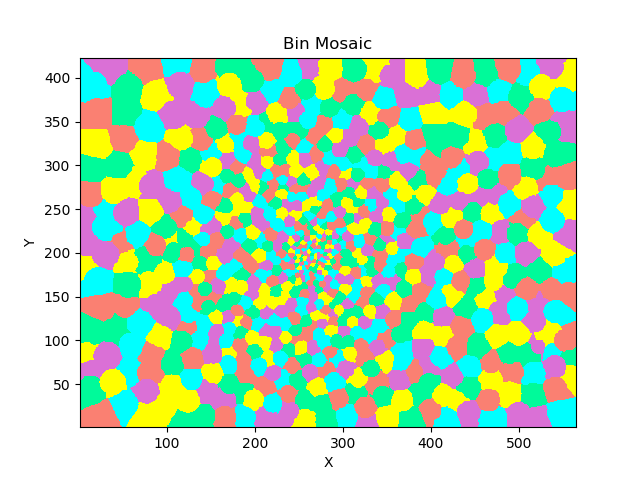
\includegraphics[width=.9\linewidth]{pictures/bin_acc}
		\caption{Bin Mosaic}
		\label{fig:sub1}
	\end{subfigure}%
	\begin{subfigure}{.5\textwidth}
		\centering
		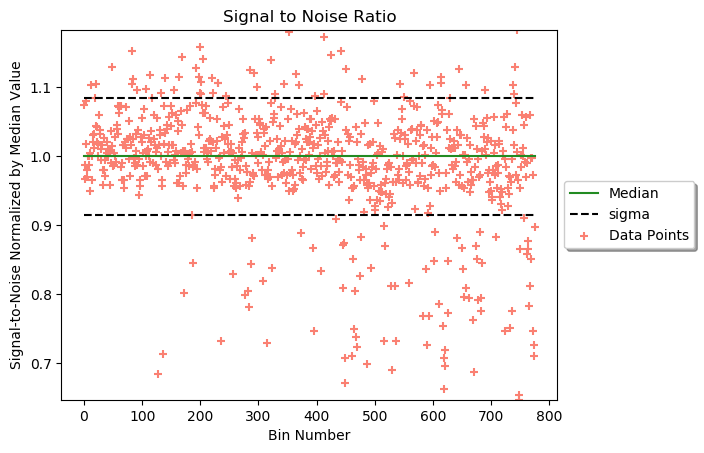
\includegraphics[width=.9\linewidth]{pictures/bin_acc_scatter}
		\caption{Signal-to-Noise Scatter}
		\label{fig:sub2}
	\end{subfigure}
	\caption{Bin Accretion Step}
	\label{fig:test}
\end{figure}
\begin{figure}
	\centering
	\begin{subfigure}{.5\textwidth}
		\centering
		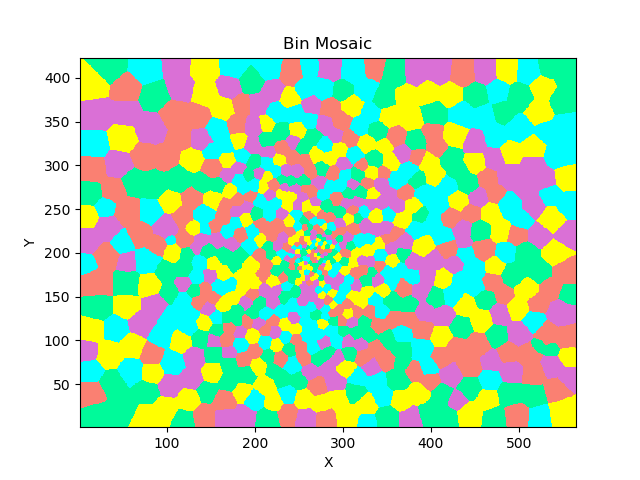
\includegraphics[width=.9\linewidth]{pictures/final}
		\caption{Bin Mosaic}
		\label{fig:sub1}
	\end{subfigure}%
	\begin{subfigure}{.5\textwidth}
		\centering
		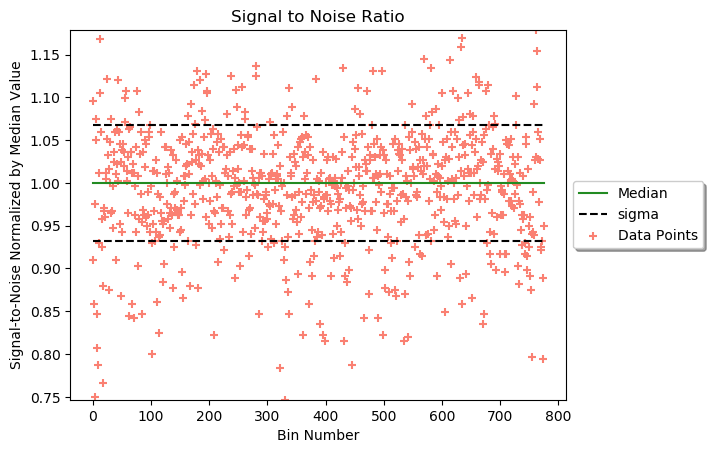
\includegraphics[width=.9\linewidth]{pictures/final_scatter}
		\caption{Signal-to-Noise Scatter}
		\label{fig:sub2}
	\end{subfigure}
	\caption{Final Step}
	\label{fig:test}
\end{figure}

\newpage
\section*{Bibliographies}
\bibliographystyle{plain}
\bibliography{bib.bib}
\end{document}